\documentclass{beamer}
\usepackage{amsfonts,amsmath,oldgerm, mathtools}
\usepackage{bm}
\usepackage{tikz}
\usepackage{booktabs}
\usepackage{hyperref}
\usetikzlibrary{calc, positioning, arrows.meta, overlay-beamer-styles, shapes.misc, decorations.pathreplacing, backgrounds}
\usetheme{dmpisa}

\renewcommand{\thefootnote}{\arabic{footnote}} % Use numeric footnote markers

\newcommand{\testcolor}[1]{\colorbox{#1}{\textcolor{#1}{test}}~\texttt{#1}}
\usefonttheme[onlymath]{serif}
\titlebackground*{assets/background} % Assicurati che il path sia corretto
\newcommand{\hrefcol}[2]{\textcolor{cyan}{\href{#1}{#2}}}

\title{Efficient Succinct Data Structures on Directed Acyclic Graphs}
\course{Tesi Triennale in Matematica}
\author{\href{mailto:l.lombardo11@studenti.unipi.it}{Luca Lombardo}} % Modifica email se necessario
\date{9 Maggio 2025}

\begin{document}

% --- SLIDE 1: Title Slide ---
\maketitle

% \section{Succinct Data structures}
% --- SLIDE 1: Titolo (Non mostrata, ma è la tua slide di titolo) ---

% --- SLIDE 2: The Subset Membership Problem ---
\begin{frame}{The Subset Membership Problem}
    \framesubtitle{Querying Collections Efficiently and Compactly}

    Consider a large universe of items $U = \{1, \dots, n\}$, and a specific subset $S \subseteq U$ of $m$ items.

    \begin{alertblock}{Core Task \& Desired Properties}
        \begin{itemize}
            \item Quickly answer: "Is item $x$ in $S$?" (\textbf{Membership Query})
            \item Store $S$ using minimal space (\textbf{Compact Representation})
        \end{itemize}
    \end{alertblock}
    \pause % Pausa prima del ponte a Shannon

    To understand "minimal space", we turn to Information Theory.
    \textit{What is the least number of bits needed to uniquely identify $S$?}
    \begin{definition}[Shannon Entropy $H(X)$]
        The average uncertainty, or information content, per symbol of source $X$:
        \[ H(X) = E_{P_X}[-\log_2 P_X(x)] = -\sum_{x \in \mathcal{X}} P_X(x) \log_2 P_X(x) \quad [\text{bits/symbol}] \]
    \end{definition}
\end{frame}

% --- SLIDE 3: Information-Theoretic Limits for Subsets ---
\begin{frame}{Information-Theoretic Limits for Subsets}
    \framesubtitle{From General Entropy to Specific Subsets}
    We usually don't know the true source $P_X$. We only have the data sequence $S$.
    \pause
    \begin{definition}[Zero-Order Empirical Entropy $\mathcal{H}_0(S)$]
        Information content of sequence $S$ based on its symbol counts ($n_s$):
        \[ \mathcal{H}_0(S) = \sum_{s \in \Sigma} \frac{n_s}{n} \log_2 \frac{n}{n_s} \quad [\text{bits/symbol}] \]
        \vspace{-0.2em}
        Uses observed frequencies $\frac{n_s}{n}$ instead of unknown $P_X(x)$.
    \end{definition}

    \pause % Pausa 2
    For our subset $S$ of $m$ items from $n$:
    \begin{itemize}
        \item There are $\binom{n}{m}$ such distinct subsets.
        \item To uniquely identify one, we need at least $\lceil \log_2 \binom{n}{m} \rceil$ bits. This is the \alert{information content} of specifying the subset.
    \end{itemize}

\end{frame}

% --- SLIDE 4: Bitvectors: Querying the Implicit Representation ---
\begin{frame}{Bitvectors: Querying the Implicit Representation}
    \framesubtitle{From Compact Storage to Element Access}

    We can represent our subset $S$ as a \textbf{bitvector} $B[1..n]$ ($B[i]=1 \iff i \in S$). We are \textbf{encoding the choice of $m$ positions for the '1's}, allowing us to store $B$ using $\approx \lceil \log_2 \binom{n}{m} \rceil$ bits. \textit{This means $B$ is not stored as an explicit array of $n$ bits.}

    % Immagine: gestita con \only per cambiare con le pause del testo
    \begin{figure}[htbp]
        \centering
        \only<1-3>{\includegraphics[width=0.95\textwidth]{assets/rank_select_1.pdf}} % Stati 1, 2, 3
        \only<4-5>{\includegraphics[width=0.95\textwidth]{assets/rank_select_2.pdf}}   % Stati 4, 5
        \only<6->{\includegraphics[width=0.95\textwidth]{assets/rank_select_3.pdf}}  % Stato 6 in poi
        \vspace{-0.5em} % Leggero aggiustamento verticale se necessario dopo l'immagine
    \end{figure}

    \pause % STATO 1 -> STATO 2 (appare la domanda)

    \uncover<2->{If $B$ is not explicit, how do we access $B[i]$? We use two foundational queries:}

    \pause % STATO 2 -> STATO 3 (appare def. rank)

    \begin{columns}[T, totalwidth=\textwidth] % Le colonne esistono, ma il contenuto appare in fasi
        \begin{column}{0.52\textwidth}
            \uncover<7->{ % Il blocco "Access Queries" appare per ultimo (STATO 7)
                \begin{block}{\textsf{Access} Queries}
                    $B[i] = 1 \iff \textsf{rank}_1(B, i) > \textsf{rank}_1(B, i-1)$
                \end{block}
            }
        \end{column}
        \begin{column}{0.45\textwidth}
            \begin{itemize}
                \item<3-> \textbf{\textsf{rank}}$_b(B, i)$: How many bits $b$ are in the prefix $B[1..i]$?
                    \pause % STATO 3 -> STATO 4 (immagine rank_select_2)
                \item<5-> \textbf{\textsf{select}}$_b(B, j)$: What is the position of the $j$-th occurrence of bit $b$?
                    \pause % STATO 5 -> STATO 6 (immagine rank_select_3)
            \end{itemize}
        \end{column}
    \end{columns}
\end{frame}

% --- SLIDE 5: RRR Structure: The Bitvector Solution ---
\begin{frame}{RRR Structure: The Bitvector Solution}
    \framesubtitle{$n\mathcal{H}_0(B)$ Space \& $O(1)$ Queries}
    \begin{block}{Succinct Data Structure for Bitvectors}
        \begin{itemize}
            \item \textbf{Goal:} Support $\textsf{rank}$ and $\textsf{select}$ in $O(1)$ time.
            \item \textbf{Space:} Close to the information-theoretic minimum for the bitvector.
        \end{itemize}
    \end{block}
    \pause
    \begin{theorem}[RRR Structure]
        A bitvector $B[1..n]$ with $m$ set bits can be represented using
        \[ B(n, m) + o(n) + O(\log \log n) \quad \text{bits}, \]
        where $B(n, m) = \lceil \log_2 \binom{n}{m} \rceil$, while supporting \textsf{rank} and \textsf{select} queries in $O(1)$ time.
    \end{theorem}
    \pause
    \begin{alertblock}{A Cornerstone Result}
        RRR shows that \textbf{optimal space} \emph{and} \textbf{efficient queries} are possible for subsets.
    \end{alertblock}
\end{frame}

% --- SLIDE 6: Why Succinct Data Structures? ---
\begin{frame}{Why Succinct Data Structures?}
    \framesubtitle{The General Challenge \& Goal}

    RRR is a specific solution to a general problem:
    \begin{block}{Massive Data \& Auxiliary Structures Overhead}
        Modern datasets (Science, Web, AI...) are enormous. Complex analysis demands data in RAM, but auxiliary structures (indexes, trees) needed for queries often \textbf{occupy more space than the data itself}.
        $\implies$ Fitting everything in RAM is a major bottleneck.
    \end{block}
    \pause
    \begin{columns}[T]
        \begin{column}<2->{0.45\textwidth}
            \textbf{Classic Trade-off:}
            \begin{itemize}
                \item \textit{Compression:} Minimal space, but slow/no direct queries.
                \item \textit{Traditional Data Structures:} Fast queries, but large space overhead.
            \end{itemize}
        \end{column}
        \begin{column}<3->{0.55\textwidth}
            \begin{alertblock}{The Succinct Goal: Best of Both Worlds}
                Can we achieve \textbf{both}?
                \begin{itemize}
                    \item Space \alert{near information-theoretic minimum}.
                    \item Efficient queries \alert{directly} on compact data.
                \end{itemize}
            \end{alertblock}
        \end{column}
    \end{columns}
\end{frame}


% \section{Rank \& Select}

In the preceding chapters, we explored foundational concepts related to data compression and information theory. We now transition to the domain of \emph{compressed data structures}, which are designed to store data in a compact format while still permitting efficient query operations directly on the compressed representation. This paradigm often leads to what is sometimes termed \emph{pointer-less programming}, where traditional memory pointers are eschewed in favor of structures built upon bit sequences (bitvectors) augmented with operations that implicitly handle navigation and access \cite{ferragina2023pearls}.

This chapter introduces the \emph{bitvector} as a fundamental building block in this area. We will formally define the core operations associated with bitvectors, namely \texttt{rank} and \texttt{select}, and investigate techniques to support these operations efficiently, often in constant time, while maintaining low space overhead (succinctness). Subsequently, we will delve into methods for compressing bitvectors themselves, particularly exploiting skewed distributions of bits, and discuss practical considerations for implementing these structures effectively. We will also briefly touch upon generalizations like wavelet trees for handling larger alphabets later in the thesis. The efficient implementation of rank and select on bitvectors is crucial, as they underpin numerous advanced compressed data structures used throughout computer science \cite{navarro2016compact}.


\section{Bitvectors} \label{sec:bitvectors}
Consider the following problem \cite{ferragina2023pearls}: imagine a dictionary $\mathcal{D}$ containing $n$ strings from an alphabet $\Sigma$. We can merge all strings in $\mathcal{D}$ into a single string $T[1,m]$, without any separators between them, where $m$ is the total length of the dictionary. The task is to handle the following queries:
\begin{itemize}
    \item \texttt{Read(i)}: retrieve the $i$-th string in $\mathcal{D}$.
    \item \texttt{Which\_string(x)}: find the starting position of the string in $T$, including the character $T[x]$.
\end{itemize}
The conventional solution involves employing an array of pointers $A[1, n]$ to the strings in $\mathcal{D}$, represented by their offsets in $T[1, m]$, requiring $\Theta(n \log n)$ bits. Consequently, \texttt{Read(i)} simply returns $A[i]$, while \texttt{Which\_string(x)} involves locating the predecessor of $x$ in $A$. The first operation is instantaneous, whereas the second one necessitates $O(\log n)$ time using binary search.

We can address the problem by employing a compressed representation of the offsets in $A$ via a binary array $B[1,m]$ of $m$ bits, where $B[i] = 1$ if and only if $i$ is the starting position of a string in $T$. In this case then $\texttt{Access\_string(i)}$ searches for the $i$-th $1$ in $B$, while $\texttt{Which\_string(x)}$ counts the number of $1$s in the prefix $B[1,x]$.

In modern literature this two operations are well known as \textit{rank} and \textit{select} queries, respectively.
\begin{definition}[Rank and Select]\label{def:rankselect}
    Given $B[1,n]$ a binary array of $n$ bits (a bitvector), we define the following operations:
    \begin{itemize}
        \item The \textbf{rank} of an index $i$ in $B$ relative to a bit $b$ is the number of occurrences of $b$ in the prefix $B[1,i]$. We denote it as $rank_1(i) = \sum_{j=1}^{i} B[j]$. Similarly we can compute $rank_0(i) = i - rank_1(i)$ in constant time.
        \item The \textbf{select} of the $i$-th occurrence of a bit $b$ in $B$ is the index of the $i$-th occurrence of $b$ in $B$. We denote it as $select_b(i)$. Opposite to rank, we can't derive select of $0$ from select of $1$ in constant time.
    \end{itemize}
\end{definition}

\begin{example}[Rank and Select on a plain bitvector]

\end{example}
\missingfigure[]{Example of a bitvector $B[1, 20]$ with the rank and select operations.}

As stated before, bitvectors are the fundamental piece in the implementation of compressed data structures. Therefore, an efficient implementation is crucial. In the following sections, our aim is to built structures of size $o(n)$ bits that can be added on top either the bit array or the compressed representation of $B$ to facilitate rank and select operations. We will see that will often encounter skewed distributions of $0$s and $1$s in $B$, and we will exploit this property to achieve higher order compression.

\begin{remark}
    If we try to compress bitvectors with the techniques seen in \autoref{ch:Chapter2}, we would need to encode each bit individually, requiring at least $n$ bits.
\end{remark}

\subsection{Rank} \label{subsec:rank}

In their seminal paper \cite{RRR2002} Raman et al. introduced a hierarchical succinct data structure that supports the rank operation in constant time, while only using only extra $o(n)$  bits of space. The structure is based on the idea of splitting the binary array $B[1, n]$ into big and small blocks of fixed length, and then encoding the number of bits set to $1$ in each block.

More precisely, the structure is composed of three levels: in the first one we (logically) split $B[1, n]$ into blocks of size $Z$ each, where at the beginning of each superblock we store the number (\emph{class number}) of bits set to $1$ in the corresponding block, i.e the output of the query $rank_1(i)$ for $i$ being the starting position of the block. In the second level, we split the superblocks into blocks of size $z$ bits each\footnote{For simplicity, we assume that $z$ divides $Z$} with the same meta-information stored at the beginning of each block. Finally the third level is a lookup table that is indexed by the small blocks and queried positions. In other words, for each possible small block and each possible position within that block, the lookup table stores the result of the $rank_1$ operation. This pre-computed information allows for constant time retrieval of the $rank_1$ operation results, as the result can be directly looked up in the table instead of having to be computed each time. This is the key to the efficiency of the data structure. In this way, the $i-th$ block, of size $Z$, can be accessed as
\[
    B[i \cdot Z + 1, (i+1) \cdot Z]
\]
while the small block $j$ of size $z$ in the $i-th$ superblock is
\[
    B[i \cdot Z + j \cdot z + 1, i \cdot Z + (j+1) \cdot z] \qquad \forall j \in [0, Z/z), \forall i \in [0, n/Z)
\]
We will denote with $r_i$ and call it \emph{absolute rank} the number of bits set to $1$ in the $i-th$ block, and with $r_{i,j}$ (\emph{relative rank}) the number of bits set to $1$ in the $j-th$ small block of the $i-th$ superblock. Figure \ref{fig:RRR} shows a visual representation of the RRR data structure.

\begin{figure}[h]
    \begin{flushright}
        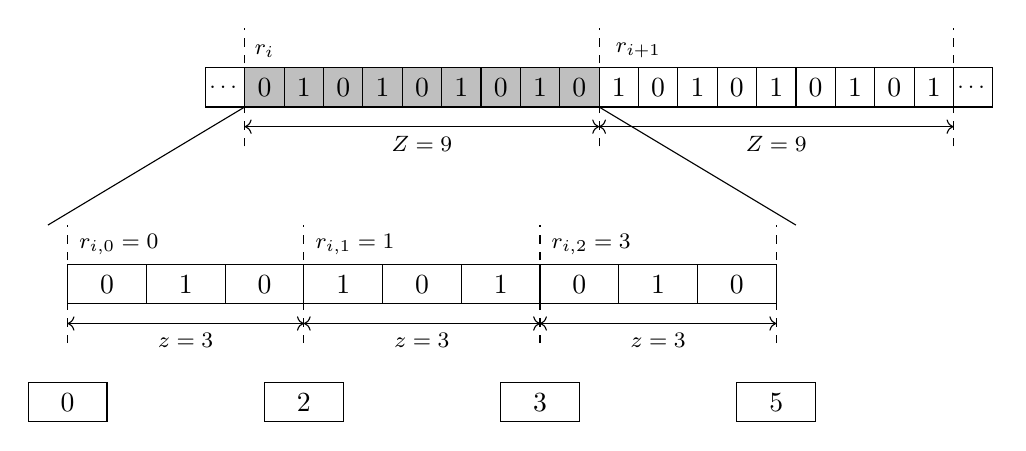
\begin{tikzpicture}[scale=0.5] % Adjust the scale as needed
            \foreach \x/\bit in {0/\footnotesize{\dots}, 1/0, 2/1, 3/0, 4/1, 5/0, 6/1, 7/0, 8/1, 9/0, 10/1, 11/0, 12/1, 13/0, 14/1, 15/0, 16/1, 17/0, 18/1, 19/\footnotesize{\dots}} {
                    \ifnum\x<1
                        \draw (\x,0) rectangle (\x+1,1) node[midway] {\bit};
                    \else
                        \ifnum\x<10
                            \draw[fill=lightgray] (\x,0) rectangle (\x+1,1) node[midway] {\bit};
                        \else
                            \draw (\x,0) rectangle (\x+1,1) node[midway] {\bit};
                        \fi
                    \fi
                }
            % Add dashed lines
            \draw[dashed] (1,-1) -- (1,2);
            \draw[dashed] (10,-1) -- (10,2);
            \draw[dashed] (19,-1) -- (19,2);

            % add double arrow
            \draw[<->] (1,-0.5) -- (10,-0.5) node[midway, below] {\footnotesize{$Z=9$}};
            \draw[<->] (10,-0.5) -- (19,-0.5) node[midway, below] {\footnotesize{$Z=9$}};

            % Add label over the blocks 2, 10
            \node[above] at (1.5,1) {\footnotesize{$r_i$}};
            \node[above] at (11,1) {\footnotesize{$r_{i+1}$}};

            % Add one line that starts from the bottom angle of block 1, and goes down inclined
            \draw[-] (1,0) -- (-4,-3);
            \draw[-] (10,0) -- (15,-3);

            \foreach \x/\bit in {0/0, 1/1, 2/0, 3/1, 4/0, 5/1, 6/0, 7/1, 8/0} {
                    \draw (\x*2-3.5,-5) rectangle (\x*2-1.5,-4) node[midway] {\bit};
                }

            % Add dashed lines
            \draw[dashed] (-3.5,-6) -- (-3.5,-3);
            \draw[dashed] (2.5,-6) -- (2.5,-3);
            \draw[dashed] (8.5,-6) -- (8.5,-3);
            \draw[dashed] (14.5,-6) -- (14.5,-3);

            % add double arrow
            \draw[<->] (-3.5,-5.5) -- (2.5,-5.5) node[midway, below] {\footnotesize{$z=3$}};
            \draw[<->] (2.5,-5.5) -- (8.5,-5.5) node[midway, below] {\footnotesize{$z=3$}};
            \draw[<->] (8.5,-5.5) -- (14.5,-5.5) node[midway, below] {\footnotesize{$z=3$}};

            % Add label over the blocks 2, 10
            \node[above] at (-2.2,-4) {\footnotesize{$r_{i,0} = 0$}};
            \node[above] at (3.8,-4) {\footnotesize{$r_{i,1} = 1$}};
            \node[above] at (9.8,-4) {\footnotesize{$r_{i,2} = 3$}};


            \foreach \x/\bit in {-4.5/0, 1.5/2, 7.5/3, 13.5/5} {
                    \draw (\x,-8) rectangle (\x+2,-7) node[midway] {\bit};
                }
        \end{tikzpicture}
    \end{flushright}
    \caption{The RRR Rank data structure. The first level is composed of blocks of size $Z$, the second level of blocks of size $z$, and the third level is an entry of the lookup table.} \label{fig:RRR}
\end{figure}

Let's focus on the third level: the lookup table. Along with the value of the absolute and relative ranks, we also store an offset that serves as an index\footnote{I we imagine that the blocks are sorted lexically, the offset is position of the block in that order} into the table. To be precise, this table is a table of tables: one for each possible value of $r_i$ and $r_{i,j}$. The table $T$ is then indexed by the values of $r_i$ and $r_{i,j}$. For every possibile value of $r_i$ and $r_{i,j}$, the sub-table stores an array of prefix sums. Thus, since we have $\binom{Z}{z}$ possible values for $r_i$ and $r_{i,j}$ (and consequently entries in the considered sub-table), the lookup table has a size of $\binom{Z}{z}\log Z$ bits. In Table \ref{tab:lookup} we show an example of a lookup table for the RRR data structure.

\begin{table}[h]
    \centering
    \begin{tabular}{|c|c|c|c|}
        % \hline
        %                & \multicolumn{3}{c|}{\textbf{cumulative rank at bit index}}                                           \\
        \hline
        \textbf{block} & $\mathbf{r_{i,0}}$ & $\mathbf{r_{i,1}}$ & $\mathbf{r_{i,2}}$ \\
        \hline
        000            & 0                  & 0                  & 0                  \\
        001            & 0                  & 0                  & 1                  \\
        010            & 0                  & 1                  & 1                  \\
        011            & 0                  & 1                  & 2                  \\
        100            & 1                  & 1                  & 1                  \\
        101            & 1                  & 1                  & 2                  \\
        110            & 1                  & 2                  & 2                  \\
        111            & 1                  & 2                  & 3                  \\
        \hline
    \end{tabular}
    \caption{Example of a lookup table $T$ for the RRR data structure. The table stores the result of the rank operation for all possible small blocks with $z = 3$. The cell $T[b, r_{i,j}]$ stores the result of the rank operation for the block $b$ inside the $i-th$ superblock and the $j-th$ small block.} \label{tab:lookup}
\end{table}

We can now state the following theorem \cite{ferragina2023pearls}:

\begin{theorem} \label{th:rank}
    The space occupancy of the Rank data structure is $o(n)$ bits, and thus it is asymptotically sublinear in the size of the binary array $B[1, n]$. The Rank algorithm takes constant time in the worst case, and accesses the array $B$ only in read-mode
\end{theorem}
\begin{proof}
    The space occupancy of all the big blocks can be computed by multiplying the number of big blocks by the number of bits needed to store the \emph{absolute rank} of each block. Thus, the space occupancy of the big blocks is $O(\frac{n}{Z} \log m)$ bits, since each block can store at most $m$ bits. The same reasoning can be applied to the small blocks, which occupy $O(\frac{n}{z} \log Z)$ bits, since each block can store at most $Z$ bits. So the space complexity is
    \begin{equation}
        O\left(\frac{n}{Z} \log m + \frac{n}{z} \log Z\right)
    \end{equation}
    Let's set $Z = (\log n)^2$ and $z = 1/2 \log n$, then the space complexity becomes
    \begin{align}
         & = O\left(\frac{n}{(\log n)^2} \log m + \frac{n}{\frac{1}{2} \log n} \log (\log n)^2\right) \\
         & = O\left(\frac{n}{\log^2n} \log m + \frac{n}{\log n} \log \log n\right)                    \\
         & = O\left(\frac{n \log \log n}{\log n} \right)= o(n)
    \end{align}
\end{proof}

The $o(n)$ space complexity highlighted in Theorem~\ref{th:rank} signifies that the auxiliary structures consume asymptotically less space than the bitvector itself. Significant research effort has been dedicated to minimizing the constant factors hidden within this $o(n)$ term and understanding the inherent space-time tradeoffs. Works such as \cite{grossi2009haste} explore techniques to further reduce this redundancy, striving for implementations that are both theoretically efficient and practically performant, often achieving space bounds closer to the information-theoretic minimum $B(n,m)$ (the space needed just to represent the bitvector) plus a smaller redundancy term, especially for certain ranges of $n$ and $m$.

The current explanation of this data structure only clarifies how to respond to rank queries for indices located at the end of a block (or superblock). This can be achieved efficiently, taking constant time, either by directly accessing the value in the lookup table or by calculating the cumulative rank of preceding blocks along with the relative rank within the current block.

However, we also need to address the non-trivial case where the index $i$ is located in the middle of a block\footnote{For the sake of simplicity, we will assume that $B[x]$ is included in the $j-th$ small block of the $i-th$ superblock}. Differently from the previous case, if we want to compute the $rank_1$ operation over an arbitrary position $x$, we would need to compute $r_i + r_{i,j} + \texttt{popcount}(B_{i,j}[1,x])$, where the last term is an operation that counts the number of bits set to $1$ in the prefix $B_{i,j}[1,x]$. While the first two terms can be computed in constant time, the last term requires $O(\log n)$ time\footnote{It actually grows log-logarithmically with the size of the small blocks} in the worst case.

% \begin{remark}
%     If $z$ (the size of the small blocks) can be stored in a single memory word, the \texttt{popcount} operation can be executed efficiently using bit manipulation operations like the \texttt{count\_ones()} method in Rust\footnote{\url{https://doc.rust-lang.org/std/primitive.u64.html\#method.count\_ones}}. This approach ensures constant time execution, especially when $z$ occupies only a few memory words, allowing for the utilization of SIMD (single instruction, multiple data) operations for faster performance. \cite{ferragina2023pearls}
% \end{remark}

If the size of the small blocks doesn't fit in a single memory word, we can pre-process in our lookup table (the third level of the data structure) all the results of the \texttt{popcount} operation for all possible blocks and then use this table to answer rank queries in constant time (as shown in table \ref{tab:lookup}). Let's denote this table as $T$ and see how to use it to answer rank queries in constant time. In order to retrive the result of $\texttt{popcount}(B_{i,j}[1,x])$ we can access the table $T$ at the position $T[B_{i,j}, o]$. Where $o$ is the offset of the bit $B[x]$ in $B_{i,j}$, and $B_{i,j}$. The offset $o$ can be computed as $o = 1 + ((x-1) \mod z)$. Thus we only need to perform three atomic operations, two memory accesses and one addition, to retrieve the result of the rank operation in constant time.

Storing this table requires $O(\sqrt{n} \log \log n)$ bits\footnote{We have $2^z$ rows and $z$ columns and each cell stores a value in $[0, z]$.}, which is asymptotically sub-linear in the size of the binary array $B[1, n]$ and allows the \texttt{popcount} operation in a block of $O(\log n)$ bits in constant time. Thus, if we consider the word length as $\log n$ and still maintain the $o(n)$ space occupancy stated in \ref{th:rank}

% Replacement for Rank Practical Considerations Remark (incorporating Broadword/rank9)


% Algorithm \ref{alg:rank} shows the Rank algorithm, which takes as input the binary array $B$ and an index $i$, and returns the rank of the bit at index $i$ in $B$. For the sake of simplicity, we will use some C++ methods from the standard library: in particular, we will use the method \texttt{std::popcount}\footnote{https://en.cppreference.com/w/cpp/numeric/popcount} that returns the number of bits set to $1$ in a given integer.

% \begin{algorithm}[h]
%     \begin{algorithmic}[1]
%         \Function{Rank}{$B,i$}
%         \State $Z \gets \log^2 n$
%         \State $z \gets \frac{1}{2} \log n$
%         \State $i \gets \lfloor i / Z \rfloor$
%         \State $j \gets \lfloor i / z \rfloor$
%         \State $r_i \gets \text{absolute rank of block } i$
%         \State $r_{i,j} \gets \text{relative rank of block } j \text{ in superblock } i$
%         \State $o \gets 1 + ((i \cdot Z + j \cdot z) \mod z)$
%         \State \Return $r_i + r_{i,j} + T[B[i,j], o]$
%         \EndFunction
%     \end{algorithmic}
%     \caption{Rank Algorithm} \label{alg:rank}
% \end{algorithm}


\subsection{Select} \label{subsec:select}
The $select$ operation can be seen as the inverse of the rank operation, i.e given a binary array $B$ and an integer $i$, the $select$ operation returns the index of the $i$-th occurrence of a bit $b$ in $B$. More formally, we have that:
\[
    rank_c(B, select_c(B, i)) = i
\]
\todo{Maybe talk about monoids and how rank and select are inverses of each other}

The implementation of the select operation heavily relies on the three level data structure discussed before (\ref{subsec:rank}). The difference lies in the fact that, in this case, the bitmap $B$ doesn't get split into blocks of fixed size, but rather into blocks of variable size that are determined by the rank of the block. We start by designing the first level of the select data structure: we split the bitmap $B$ into blocks of size $Z$ bitvectors each containing $K$ bits set to $1$.

\begin{remark}[Notation and assumptions]
    In the following, $Z$ will represent, as before, the size in bits of the big blocks containing $K$ bits set to $1$, where $K = \log n$. We will use always the same notation $Z$ even if the size of the blocks is variable, clarifying the context in which it is used.
\end{remark}

Since $K \leq Z$, we can easily derive that space occupance of all the starting positions of the blocks $O(\frac{n}{K} \log n) = o(n)$ bits. The first step of our search in then clear: since each block contains $K$ bits set to $1$, we can find the block containing the $i$-th occurrence of $1$ in $B$ by computing $i/K$.

The second step is to find the $i$-th occurrence of $1$ in the block. This could be done by scanning the block from the beginning and counting the number of bits set to $1$ until we reach the $i$-th occurrence, but this would require $O(K)$ time making it highly un-efficient for our purposes. To address this issue, we introduce the second level of the select data structure where we divide the big blocks into smaller blocks and categorize them into two types: \emph{dense} and \emph{sparse} blocks. A big block is considered \emph{dense} if $Z \leq K^2$ and \emph{sparse} otherwise. When dealing with a sparse block, we can store the positions of the bits set to $1$ in the block in a separate array, allowing us to access the $i$-th occurrence of $1$ in constant time. Due to it's small number of bits set to $1$, we can store the positions in $O(\frac{n}{K^2}K \log n) = O(\frac{n}{\log^2n} \log n) = o(n)$ bits.

Dealing with the dense blocks is not as straightforward as with the sparse ones. In this case, we can't afford to store the positions of the bits set to $1$ in the block, as it would require too much space. We introduce then the third level of the select data structure, where we split the dense blocks into smaller blocks of length\footnote{The same assumptions made before apply as well: $z$ can vary but we will use the same notation for simplicity and clarify the context in which it is used idf necessary} $z$, each containing $k = (\log \log m)^2$ bits set to $1$. Thus storing all the starting positions of the smalls blocks and relative beginning of the dense blocks requires $O(\frac{n}{k} \log K^2) = O(\frac{n}{(\log \log n)^2} \log \log^4 n) = o(n)$ bits\footnote{
    We exploited the fact that each small block has at least length $k$ and the length of its enclosing dense block is at most $K^2$.
}.

The only remaining issue is to keep track of the positions of the bits set to $1$ in the small blocks. We can follow the idea introduced for the big blocks and divide them into \emph{dense} and \emph{sparse} small blocks. The sparse small blocks are those with length less then $k^2 = (\log \log m)^4$, and we can store the positions of the bits set to $1$ in the block relative to the beginning of its enclosing block in
\[
    O\left(\frac{n}{k^2} k \log K^2 \right) = O\left(\frac{n}{(\log \log n)^2} \log \log^4 n\right) = o(n)
\]
bits\footnote{
    We exploited the fact that each sparse small block has length $z > k^2$, thus their number is $O(\frac{n}{k^2})$. We also note that the length of the enclosing dense block is at most $K^2$.
}. Following the idea of the third level of the rank data structure, we can store the positions of the bits set to $1$ in the dense small blocks in a lookup table, allowing us to access the $i$-th occurrence of $1$ in constant time. This table will store all the pre-computed results of the select operation for all possible small blocks and, since $z \leq k^2$, having $2^z$ columns and $z$ rows, it will require $O(z 2^z \log z) = o(n)$ bits\footnote{
    Each cell of the table stores a value in $[0, z]$, thus the $\log z$ factor.
}.

\begin{remark}[Pratical Considerations]
    The value $(\log log m)^4$ can be very small for practical values of $m$, thus we could avoid dividing the small blocks into dense and sparse blocks and just scan the block from the beginning to find the $i$-th occurrence of $1$.
\end{remark}

In algorithm \ref{alg:select} are outlined the steps of the $select_1$ (the $select_0$ works in the same way) algorithm, which takes as input the binary array $B$ and an index $i$, and returns the index of the $i$-th occurrence of a bit $b$ in $B$.

\begin{algorithm}[hbtp]
    \caption{$Select_1$ Algorithm} \label{alg:select}
    \begin{algorithmic}
        \Function{$Select_1$}{$B, i$}
        \State $ j = 1 + \lfloor \frac{i-1}{K} \rfloor$ \Comment{\small{index of big block}}
        \State $B_{j} \gets$ big block $j$
        \If{$B_{j}$ \emph{is sparse}}
        \State $S \gets$ array of positions of bits set to $1$ in $B_{j}$
        \State \Return $S[i \mod K]$
        \Else
        % the data structure has stored the staring position of the dense big block B_j, say s_j
        \State $s_j \gets$ starting position of $B_{j}$
        \State $i' \gets 1 + (i-1 \mod K)$ \Comment{\small{Relative $select$ index in the block}}
        \State $j' \gets 1 + \lfloor \frac{i'-1}{k} \rfloor$ \Comment{\small{index of small block}}
        \State $B_{j,j'} \gets$ small block $j'$ in big block $j$
        % the data structure has stored the staring position of the dense small block B_{j,j'}, say s_{j,j'}
        \State $s_{j,j'} \gets$ starting position of $B_{j,j'}$
        \If{$B_{j,j'}$ \emph{is sparse}}
        \State $S \gets$ array of positions of bits set to $1$ in $B_{j,j'}$
        \State \Return $s_j + S[i' \mod k]$
        \Else
        % we access the lookup table T with values B_{j,j'} and 1 + (i+1 \mod k^2), and we get the answer to the select query by summig s_j + s_j' + T[B_{j,j'}, 1 + (i+1 \mod k^2)]
        \State $o \gets 1 + (i'-1 \mod k^2)$ \Comment{\small{offset in the small block}}
        \State \Return $s_j + s_{j,j'} + T[B_{j,j'}, o]$
        \EndIf
        \EndIf
        \EndFunction
    \end{algorithmic}
\end{algorithm}

As for the rank data structure, we can state the following theorem:

\begin{theorem} \label{th:select}
    The space occupancy of the Select data structure is $o(n)$ bits, and thus it is asymptotically sublinear in the size of the binary array $B[1, n]$. The Select algorithm takes constant time in the worst case, and accesses the array $B$ only in read-mode
\end{theorem}
\begin{proof}
    Follows from the previous discussion.
\end{proof}
For dense small blocks whose size $z$ is very small (e.g., $z \le k^2 = (\log \log m)^4$), direct scanning can indeed be faster than accessing the precomputed table $T$.


\subsection{Compressing Sparse Bitvectors with Elias-Fano} \label{subsec:elias_fano_compression}

The rank and select structures discussed before (\ref{subsec:rank}, \ref{subsec:select}) operate on the plain bitvector $B[1,n]$, achieving a total space occupancy of $n + o(n)$ bits. However, in many practical scenarios, the bitvector $B$ exhibits a skewed distribution, containing significantly fewer 1s than 0s (or vice-versa). Let $m = rank_1(n)$ be the total number of set bits. When $m \ll n$, storing the full $n$-bit vector is inefficient.

In such sparse settings, we can leverage compression techniques that exploit the low density of set bits. The Elias-Fano representation, previously introduced in Section~\ref{sec:elias_fano_code}, provides a highly effective method for this task. Recall that Elias-Fano encodes a monotonically increasing sequence of $m$ integers up to a maximum value $n$. We can represent the bitvector $B$ by encoding the sequence of indices $\{ i \mid B[i]=1 \}$.

As detailed by Vigna \cite{vigna2013quasi} in the context of quasi-succinct indices for information retrieval, the Elias-Fano representation achieves a space complexity of approximately $m \log_2(n/m) + O(m)$ bits. This is remarkably close to the information-theoretic lower bound for representing a subset of size $m$ from a universe of size $n$, often expressed as $n\mathcal{H}_0(B) + O(m)$ bits, where $\mathcal{H}_0(B)$ is the empirical zero-order entropy of the bitvector $B$. The crucial advantage is that the space depends primarily on $m$, the number of set bits, rather than the full length $n$, leading to significant compression when $m$ is small.

This compressed representation directly supports efficient operations. The $select_1(i)$ operation, finding the position of the $i$-th set bit, can typically be implemented in constant time on average, often leveraging auxiliary pointers within the Elias-Fano structure as engineered in \cite{vigna2013quasi}. However, this space efficiency comes at the cost of potentially slower $rank_1$ and $access$ (checking the value of $B[i]$) operations compared to the $n+o(n)$ structures. These operations usually involve decoding parts of the Elias-Fano structure and may take $O(\log(n/m))$ time or depend on the specific implementation details \cite{navarro2016compact}. Therefore, Elias-Fano presents a compelling space-time trade-off, offering near-optimal compression for sparse bitvectors at the expense of rank and access time complexity. The choice between plain bitvector structures and Elias-Fano depends critically on the sparsity of the data and the required query performance profile.

\subsection{Practical Implementation Considerations} \label{subsec:practical_considerations}

While the asymptotic analysis guarantees $O(1)$ query time and $o(n)$ extra space for the rank and select structures presented earlier, achieving high performance in practice requires careful consideration of architectural factors and constant overheads hidden in the $o(n)$ term. Memory latency, cache efficiency, and instruction-level parallelism often dominate the actual running time on modern processors \cite{ferragina2023pearls}.

A particularly effective approach for optimizing rank and select implementations leverages \emph{broadword programming} (also known as \textsc{Swar} - \textsc{Simd} Within A Register). This technique treats machine registers as small parallel processors, performing operations on multiple data fields packed within a single word using standard arithmetic and logical instructions. Vigna \cite{vigna2008broadword} applied these techniques to rank and select queries, leading to highly efficient practical implementations.

The \texttt{rank9} structure proposed by Vigna \cite{vigna2008broadword} exemplifies this approach. It employs a two-level hierarchy, similar in concept to the structure in Section~\ref{subsec:rank}, but critically relies on broadword algorithms for the final rank computation within a machine word (specifically, sideways addition or population count). Instead of large precomputed lookup tables for small blocks, \texttt{rank9} uses carefully designed constants and bitwise operations (detailed in Algorithm 1 of \cite{vigna2008broadword}) to compute the rank within a 64-bit word quickly. This typically involves storing relative counts for sub-blocks (e.g., seven 9-bit counts within a 64-bit word) in the second level. The advantages include:
\begin{itemize}
    \item Speed: Exploits fast register operations and avoids large table lookups, often outperforming other methods in practice.
    \item Space Efficiency: Requires relatively low space overhead, typically around 25\% on top of the original bitvector $B$, mainly for storing the cumulative rank counts.
    \item Branch Avoidance: Broadword algorithms are generally branch-free, which benefits performance on modern pipelined processors by avoiding potential misprediction penalties.
\end{itemize}

Similarly, Vigna \cite{vigna2008broadword} developed broadword algorithms for selection within a word (Algorithm 2 in the paper). The companion \texttt{select9} structure integrates these intra-word selection capabilities with a multi-level inventory scheme. The objective of \texttt{select9} is to support high-performance selection queries, often achieving near constant-time execution, through hierarchical indexing combined with efficient broadword search for the final location. This capability involves an additional space cost, typically measured at approximately 37.5\% relative to the \texttt{rank9} structure.

Furthermore, a major bottleneck in rank/select operations is often memory access latency. To mitigate this, \emph{interleaving} the auxiliary data structures is highly recommended. For instance, storing a first-level (superblock) rank count immediately followed by its corresponding second-level (sub-block) counts increases the probability that all necessary auxiliary information for a query resides within the same cache line. This simple layout optimization can dramatically reduce cache misses compared to storing different levels of the hierarchy in separate arrays.


% \subsection{Strings}

% --- SLIDE 7: Beyond Bits: General Alphabets ---
\begin{frame}{Beyond Bitvectors: General Alphabets}
    \framesubtitle{Wavelet Trees}
    \vspace{-0.2em}
    What about sequences $S[1..n]$ over larger alphabets $\Sigma = \{1, \dots, \sigma\}$?
    \begin{figure}[hbtp]
        \centering
        \only<2>{\includegraphics[width=0.6\textwidth]{assets/wt1.pdf}} % Visible only on slide 2
        \only<3>{\includegraphics[width=0.7\textwidth]{assets/wt2.pdf}} % Visible only on slide 3
        \only<4>{\includegraphics[width=\textwidth]{assets/wt3.pdf}} % Visible only on slide 4
        \only<5>{\includegraphics[width=0.7\textwidth]{assets/wt4.pdf}} % Visible ONLY on slide 5
    \end{figure}
    \only<6->{
        \begin{columns}[T] % Align columns at the top
            \begin{column}{0.55\textwidth} % Adjust width as needed
                \centering % Center the image in the column
                \includegraphics[width=\textwidth]{assets/wt4.pdf} % Show from slide 6 onwards
            \end{column}
            \begin{column}{0.45\textwidth} % Adjust width as needed
                \begin{block}{$\mathcal{H}_0$-Compressed Wavelet Tree} % Ref Thm 3.8 in thesis
                    Using RRR for bitvectors:
                    \begin{itemize}
                        \item \textbf{Space}: $n \mathcal{H}_0(S) + o(n \log \sigma)$ bits.
                        \item \textbf{Query Time}: $O(\log \sigma)$ for \textsf{access}, \textsf{rank}$_c$, \textsf{select}$_c$.
                    \end{itemize}
                    Adapts space to the sequence's zero-order entropy.
                \end{block}
            \end{column}
        \end{columns}
    }
\end{frame}

% \begin{frame}{Wavelet Tree Construction: Example}
%     \framesubtitle{Step 1: Splitting the Root}
%     \begin{columns}[T,totalwidth=\textwidth] % Colonne allineate in alto
%         % Colonna sinistra: Spiegazioni
%         \begin{column}{0.5\textwidth}
%             % Spazio sopra allineato con l'alfabeto a destra
%             \vspace*{1ex} % Aggiusta se necessario

%             \uncover<1->{
%                 \textbf{1. Alphabet Split:}
%                 \begin{itemize}
%                     \item Root covers $\Sigma = \{\texttt{a, b, c, d, r}\}$.
%                     \item Use range $[1, 5]$.
%                     \item Midpoint $m = 3$ is \alert{c}.
%                     \item Split into: $[\texttt{a, b, c}]$ vs $[\texttt{d, r}]$.
%                 \end{itemize}
%                 \bigskip
%             }
%             \uncover<2->{
%                 \textbf{2. Bitmap Rule ($B_{root}$):}
%                 \begin{itemize}
%                     \item If char $\le$ \alert{c} $\rightarrow$ Bit \textcolor{blue!70!black}{0} (Goes Left)
%                     \item If char $>$ \alert{c} $\rightarrow$ Bit \textcolor{red!70!black}{1} (Goes Right)
%                 \end{itemize}
%                 \bigskip
%             }
%         \end{column}

%         % Colonna destra: Visualizzazione
%         \begin{column}{0.5\textwidth}
%             \centering
%             % Spazio sopra allineato con l'alfabeto a sinistra
%             \vspace*{9ex} % Aggiusta se necessario

%             % Visualizzazione dell'alfabeto
%             \uncover<2->{\includegraphics[width=0.5\textwidth]{../bachelor-thesis/TeX/assets/WT_slides_root.pdf}} % Mostra solo quando necessario
%         \end{column}
%     \end{columns}
% \end{frame}

% \begin{frame}{Wavelet Tree Construction: Example}
%     \framesubtitle{Building the Tree}
%     \begin{figure}[hbtp]
%         \centering
%         % Replace TikZ with sequential images
%         \only<1>{\includegraphics[width=0.7\textwidth]{../bachelor-thesis/TeX/assets/WT_slides1.pdf}} % Visible only on slide 2
%         \only<2>{\includegraphics[width=0.7\textwidth]{../bachelor-thesis/TeX/assets/WT_slides2.pdf}} % Visible only on slide 3
%         \only<3->{\includegraphics[width=0.7\textwidth]{../bachelor-thesis/TeX/assets/WT_slides3.pdf}} % Visible from slide 4 onwards
%         % \caption{Hierarchical structure for Rank}
%     \end{figure}
% \end{frame}

% \begin{frame}{Wavelet Tree: Rank Example}
%     \framesubtitle{Rank on Wavelet Trees}

%     \begin{figure}[hbtp]
%         \centering
%         % Replace TikZ with sequential images
%         \only<1>{\includegraphics[width=0.7\textwidth]{../bachelor-thesis/TeX/assets/WT_rank_slides1.pdf}} % Visible only on slide 2
%         \only<2>{\includegraphics[width=0.7\textwidth]{../bachelor-thesis/TeX/assets/WT_rank_slides2.pdf}} % Visible only on slide 3
%         \only<3->{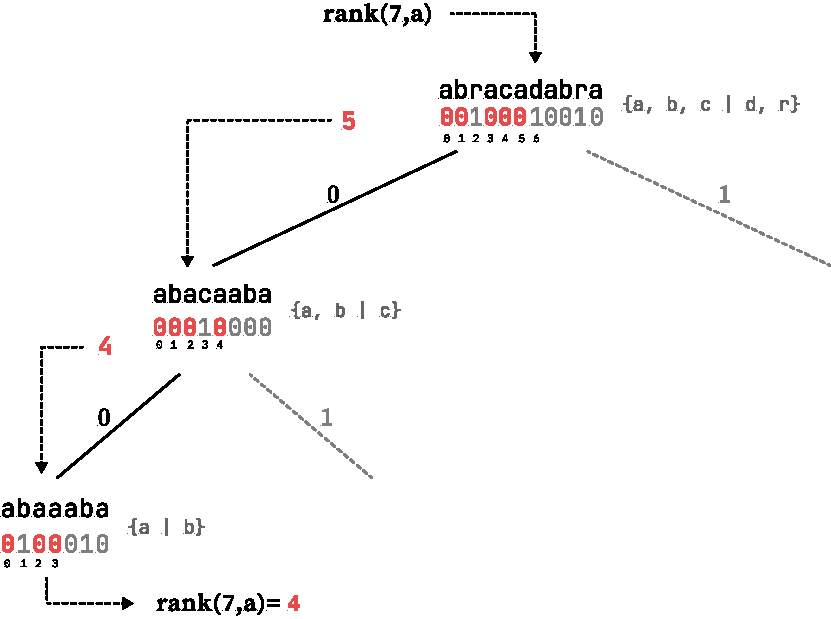
\includegraphics[width=0.65\textwidth]{../bachelor-thesis/TeX/assets/WT_rank_slides3.pdf}} % Visible from slide 4 onwards
%         % \caption{Hierarchical structure for Rank}
%     \end{figure}
% \end{frame}

% % --- SLIDE 8: Wavelet Tree Performance Summary ---
% \begin{frame}{Wavelet Tree: Performance Summary}
%     \framesubtitle{Space and Query Time}

%     % Standard WT Result
%     \begin{theorem}[Standard Wavelet Tree]
%         Represents $S[1..n]$ over $\Sigma=\{1,\dots,\sigma\}$ using:
%         \begin{itemize}
%             \item \textbf{Space}: $n \lceil \log \sigma \rceil + o(n \log \sigma)$ bits.
%             \item \textbf{Query Time}: $O(\log \sigma)$ for \textsf{access}, \textsf{rank}$_c$, \textsf{select}$_c$.
%         \end{itemize}
%     \end{theorem}

%     \pause % Introduce compressed versions

%     % Compressed WT (H0)
%     \begin{theorem}[$\mathcal{H}_0$-Compressed Wavelet Tree] % Ref Thm 3.8 in thesis
%         Using RRR for bitvectors:
%         \begin{itemize}
%             \item \textbf{Space}: $n \mathcal{H}_0(S) + o(n \log \sigma)$ bits.
%             \item \textbf{Query Time}: $O(\log \sigma)$ for \textsf{access}, \textsf{rank}$_c$, \textsf{select}$_c$.
%         \end{itemize}
%         Adapts space to the sequence's zero-order entropy.
%     \end{theorem}
% \end{frame}


% \subsection{Degenerate Strings}

% --- SLIDE 9: Degenerate Strings ---
\begin{frame}{Representing Sequence Variation: Degenerate Strings}
    \framesubtitle{Definitions and Core Operations}
    \begin{block}{Definition and Rank \& Select Adaptation}
        A \textbf{degenerate string} is a sequence $X = X_1 X_2 \dots X_n$, where each $X_i$ is a \emph{subset} of the alphabet $\Sigma$ with cardinality $\sigma$. We can define the following operations:
        \begin{itemize}
            \item \textsf{subset-rank}$_X(i, c)$: Counts sets $X_k$ ($k \le i$) where $c \in X_k$.
            \item \textsf{subset-select}$_X(j, c)$: Finds index $k$ of the $j$-th set $X_k$ where $c \in X_k$.
        \end{itemize}
    \end{block}
    \pause
    \begin{figure}[h!] % Nota: [h!] può essere problematico, [htbp] è più sicuro
        \centering
        \begin{tabular}{c@{\hskip 0.5em}c@{\hskip 0.5em}c@{\hskip 0.5em}c@{\hskip 0.5em}c}
            $X = $                                                               & $\Bigg\{\,\begin{matrix}\texttt{A}\\\texttt{C}\\\texttt{G}\end{matrix}\,\Bigg\}$ &
            $\Bigg\{\,\begin{matrix}\texttt{A}\\\texttt{T}\end{matrix}\,\Bigg\}$ &
            $\Bigg\{\,\begin{matrix}\texttt{C}\end{matrix}\,\Bigg\}$             &
            $\Bigg\{\,\begin{matrix}\texttt{T}\\\texttt{G}\end{matrix}\,\Bigg\}$                                                                                                            \\
                                                                                 & $X_1$                                                                            & $X_2$ & $X_3$ & $X_4$
        \end{tabular}
        \uncover<2->{\qquad
            \begin{tabular}{c@{\hskip 0.5em}c@{\hskip 0.5em}c@{\hskip 0.5em}c@{\hskip 0.5em}c@{\hskip 0.5em}c}
                $S =$  & \texttt{ACG} & \texttt{AT} & \texttt{C} & \texttt{TG} &            \\
                $R = $ & \texttt{100} & \texttt{10} & \texttt{1} & \texttt{10} & \texttt{1} \\
                       & $S_1$        & $S_2$       & $S_3$      & $S_4$
            \end{tabular}
        }
    \end{figure}
    % --- Paragrafo Riscritto ---
    \uncover<3->{% Potrebbe essere utile per far apparire il testo solo al terzo step
        To compute \textsf{subset-rank}$_X(i, c)$: Let $p$ be the end position in $S$ for prefix $X_1..X_i$, found using $\textsf{select}_1(R, i+1)$. The result is $\textsf{rank}_c(S, p)$.
    }
\end{frame}

% % --- SLIDE 10: Degenerate Strings: Space Complexity Results ---
% \begin{frame}{Degenerate Strings: Space Complexity}
%     \framesubtitle{Reduction-Based Approach}

%     % Recall the reduction converts $X$ (length $n$, size $N$) into $S$ (length $N$) and $R$ (length $N+1$).

%     % Blocco 1: Componenti Spazio
%     \begin{block}<1->{Space Components}
%         % The total space depends on:
%         \begin{itemize}
%             \item Storing string $S$: Requires a structure $\mathcal{D}$ supporting \textsf{rank}$_c$/\textsf{select}$_c$.
%             \item Storing bitvector $R$: Requires a structure $\mathcal{V}$ supporting \textsf{rank}/\textsf{select}
%         \end{itemize}
%     \end{block}

%     % Blocco 2: Risultato Generale (Caso n0=0)
%     \begin{block}<2->{Upper Bound (No Empty Sets)}
%         % If $X$ has no empty sets ($n_0 = 0$):
%         \begin{itemize}
%             \item Total Space: $\underbrace{\mathcal{D}_b(N, \sigma)}_{\text{Space for } S} + \underbrace{N + o(N)}_{\text{Space for } R \text{ (succinct)}}$ bits.
%             \item Using standard succinct structures (e.g., Wavelet Tree for $S$, RRR for $R$): Space becomes $\approx N \log \sigma + N + o(N \log \sigma)$ bits.
%         \end{itemize}
%     \end{block}

%     \uncover<3->{\textbf{Lower Bound}: Any structure supporting \texttt{subset-rank} or \texttt{subset-select} requires at least $N \log \sigma - o(N \log \sigma)$ bits in the worst case.}

% \end{frame}


% \section{Path Queries on DAGs}
% \subsection{Path Queries}
% --- SLIDE 11: Connecting Degenerate Strings to DAGs ---
\begin{frame}{From Degenerate Strings to Weighted DAGs}
    \framesubtitle{A New Perspective}

    Recall our degenerate string $X$:
    \begin{figure}[h!]
        \centering
        % Usa la figura della stringa degenere che hai già definito
        \begin{tabular}{c@{\hskip 0.5em}c@{\hskip 0.5em}c@{\hskip 0.5em}c@{\hskip 0.5em}c}
            $X = $                                                                           & $\Bigg\{\,\begin{matrix}\texttt{A}\\\texttt{C}\\\texttt{G}\end{matrix}\,\Bigg\}$ &
            $\Bigg\{\,\begin{matrix}\texttt{A}\\\texttt{T}\end{matrix}\,\Bigg\}$             &
            $\Bigg\{\,\begin{matrix}\texttt{T}\\\texttt{C}\\\texttt{A}\end{matrix}\,\Bigg\}$ &
            $\Bigg\{\,\begin{matrix}\texttt{A}\\\texttt{G}\end{matrix}\,\Bigg\}$                                                                                                                        \\
                                                                                             & $X_1$                                                                            & $X_2$ & $X_3$ & $X_4$
        \end{tabular}
    \end{figure}

    \uncover<2->{
        \begin{block}{Key Idea}
            We can model queries on $X$ by constructing a specific node-weighted Directed Acyclic Graph (DAG) $G_c$ for a target character $c$.
        \end{block}
    }

    \uncover<3->{
        \begin{itemize}
            \item<3-> \textbf{Vertices $V_c$}: Source $s$ + one node $v_{k,a}$ for each character $a \in X_k$ at each position $k$.
            \item<4-> \textbf{Weights $w_c$}: $w_c(s)=0$. $w_c(v_{k,a}) = 1$ if $a = c$, else $0$. (Highlights occurrences of $c$).
            \item<5-> \textbf{Edges $E_c$}: Connect $s$ to $k=1$. Connect all $v_{k,a}$ to all $v_{k+1,b}$. (Represents sequence adjacency).
        \end{itemize}
    }

\end{frame}

% % --- SLIDE 12: Visualizing the DAG Construction (Example: c = A) --- USING \pause
% \begin{frame}{Visualizing the DAG Construction (Example: c = A)}
%     \framesubtitle{Building $G_A$ Step-by-Step}

%     \begin{figure}[h!]
%         \centering
%         \resizebox{\textwidth}{!}{% Resize to fit slide width if needed
%             \begin{tikzpicture}[
%                     node distance=2.8cm and 1.0cm, % x distance and y distance
%                     % Define node styles explicitly for clarity
%                     node_style/.style={circle, draw, thick, minimum size=7mm, inner sep=0pt},
%                     weight_one/.style={node_style, fill=yellow!50},
%                     weight_zero/.style={node_style, fill=gray!20},
%                     source_node/.style={node_style, fill=red!60},
%                     % Edge style
%                     edge_style/.style={->, >=latex, thin, gray}
%                 ]

%                 % --- Step 1: Draw Source Node ---
%                 \node[source_node] (s) at (0, 0) {$s$};

%                 % --- Step 2: Draw Level 1 Nodes and Edges from s ---
%                 \node[weight_one] (v1A) at (2, 2) {\tiny (1,A)}; \node[below=1pt of v1A] {\tiny w=1};
%                 \node[weight_zero](v1C) at (2, 0) {\tiny (1,C)}; \node[below=1pt of v1C] {\tiny w=0};
%                 \node[weight_zero](v1G) at (2,-2) {\tiny (1,G)}; \node[below=1pt of v1G] {\tiny w=0};
%                 \foreach \v in {v1A, v1C, v1G} { \draw[edge_style] (s) -- (\v); }

%                 \pause % Wait for click

%                 % --- Step 3: Draw Level 2 Nodes and Edges from Level 1 ---
%                 \node[weight_one] (v2A) at (4.8, 1) {\tiny (2,A)}; \node[below=1pt of v2A] {\tiny w=1};
%                 \node[weight_zero](v2T) at (4.8,-1) {\tiny (2,T)}; \node[below=1pt of v2T] {\tiny w=0};
%                 \foreach \u in {v1A, v1C, v1G} {
%                         \foreach \v in {v2A, v2T} { \draw[edge_style] (\u) -- (\v); }
%                     }

%                 \pause % Wait for click

%                 % --- Step 4: Draw Level 3 Nodes and Edges from Level 2 ---
%                 \node[weight_zero] (v3T) at (7.6, 2) {\tiny (3,T)}; \node[below=1pt of v3T] {\tiny w=0};
%                 \node[weight_zero](v3C) at (7.6, 0) {\tiny (3,C)}; \node[below=1pt of v3C] {\tiny w=0};
%                 \node[weight_one](v3A) at (7.6,-2) {\tiny (3,A)}; \node[below=1pt of v3A] {\tiny w=1};
%                 \foreach \u in {v2A, v2T} {
%                         \foreach \v in {v3T, v3C, v3A} { \draw[edge_style] (\u) -- (\v); }
%                     }

%                 \pause % Wait for click

%                 % --- Step 5: Draw Level 4 Nodes and Edges from Level 3 ---
%                 \node[weight_one] (v4A) at (10.4, 1) {\tiny (4,A)}; \node[below=1pt of v4A] {\tiny w=1};
%                 \node[weight_zero](v4G) at (10.4,-1) {\tiny (4,G)}; \node[below=1pt of v4G] {\tiny w=0};
%                 \foreach \u in {v3T, v3C, v3A} {
%                         \foreach \v in {v4A, v4G} { \draw[edge_style] (\u) -- (\v); }
%                     }

%             \end{tikzpicture}
%         } % End resizebox
%     \end{figure}

%     % Il testo finale appare dopo l'ultimo pause implicito
%     \begin{center}
%         This connection motivates the core topic: \\ \textbf{Efficient data structures for path-based queries on general node-weighted DAGs.}
%     \end{center}

% \end{frame}


% \begin{frame}{Mathematical Framework: Weighted DAGs}
%     \framesubtitle{Basic Definitions}
%     Given a path $P=(v_0=s, \dots, v_k=v)$ we define $W(P) = \sum_{j=1}^{k} w(v_j)$ as the cumulative weight of the path $P$.
%     % \begin{block}{Path and Path Weight}
%     %     \begin{itemize}
%     %         \item Path $P = (v_0=s, \dots, v_k=v)$.
%     %         \item Weight $W(P) = \sum_{j=1}^{k} w(v_j)$.
%     %     \end{itemize}
%     % \end{block}
%     \begin{figure}[h!]
%         \centering
%         \resizebox{0.95\textwidth}{!}{% Scale to fit column
%             \begin{tikzpicture}[
%                 node distance=1.5cm and 1cm,
%                 base_node/.style={circle, draw=black, thick, minimum size=8mm, inner sep=0pt, font=\sffamily},
%                 root_node/.style={base_node, fill=red!60, text=black},
%                 edge_style/.style={->, >={Stealth[length=2mm]}, thick, draw=black}
%                 ]
%                 % Nodes showing only their weight w(v)
%                 \node[root_node] (0) at (0, 2) {0};
%                 \node[base_node] (1) at (1.5, 0) {1};
%                 \node[base_node] (3) at (1.5, 4) {3};
%                 \node[base_node] (6) at (3.5, 1.5) {6};
%                 \node[base_node] (7) at (4.5, 0) {7};
%                 \node[base_node] (2) at (5.5, 4) {2};
%                 \node[base_node] (9) at (6.5, 2) {9};
%                 \node[base_node] (5) at (9, 0.5) {5};
%                 \node[base_node] (10) at (8.5, 5) {10};
%                 \node[base_node] (8) at (11, 3) {8};

%                 % Edges (same as before)
%                 \draw [edge_style] (0) -- (1); \draw [edge_style] (0) -- (3);
%                 \draw [edge_style] (1) -- (6); \draw [edge_style] (1) -- (7);
%                 \draw [edge_style] (3) -- (2); \draw [edge_style] (3) -- (6);
%                 \draw [edge_style] (6) -- (2); \draw [edge_style] (6) -- (9);
%                 \draw [edge_style] (7) -- (5); \draw [edge_style] (7) -- (9);
%                 \draw [edge_style] (2) -- (10);
%                 \draw [edge_style] (9) -- (5); \draw [edge_style] (9) -- (8);
%                 \draw [edge_style] (10) -- (8); \draw [edge_style] (5) -- (8);
%             \end{tikzpicture}
%         } % End resizebox
%     \end{figure}

%     % \begin{columns}[T]
%     %     % Colonna sinistra: Definizioni
%     %     \begin{column}{0.5\textwidth}
%     %         \begin{block}{Weighted DAG $G=(V, E, w)$}
%     %             \begin{itemize}
%     %                 \item $V$: Finite set of vertices.
%     %                 \item $E$: Directed edges, no cycles.
%     %                 \item $w: V \to \mathbb{N}_0$: Non-negative node weights.
%     %                 \item Unique source $s$ with $w(s)=0$.
%     %             \end{itemize}
%     %         \end{block}
%     %         \begin{block}{Path and Path Weight}
%     %             \begin{itemize}
%     %                 \item Path $P = (v_0=s, \dots, v_k=v)$.
%     %                 \item Weight $W(P) = \sum_{j=1}^{k} w(v_j)$.
%     %             \end{itemize}
%     %         \end{block}
%     %     \end{column}

%     %     % Colonna destra: Figura Esempio DAG (solo pesi)
%     %     \begin{column}{0.5\textwidth}
%     %         \begin{figure}[h!]
%     %             \centering
%     %             \resizebox{0.95\textwidth}{!}{% Scale to fit column
%     %                 \begin{tikzpicture}[
%     %                     node distance=1.5cm and 1cm,
%     %                     base_node/.style={circle, draw=black, thick, minimum size=8mm, inner sep=0pt, font=\sffamily},
%     %                     root_node/.style={base_node, fill=red!60, text=black},
%     %                     edge_style/.style={->, >={Stealth[length=2mm]}, thick, draw=black}
%     %                     ]
%     %                     % Nodes showing only their weight w(v)
%     %                     \node[root_node] (0) at (0, 2) {0};
%     %                     \node[base_node] (1) at (1.5, 0) {1};
%     %                     \node[base_node] (3) at (1.5, 4) {3};
%     %                     \node[base_node] (6) at (3.5, 1.5) {6};
%     %                     \node[base_node] (7) at (4.5, 0) {7};
%     %                     \node[base_node] (2) at (5.5, 4) {2};
%     %                     \node[base_node] (9) at (6.5, 2) {9};
%     %                     \node[base_node] (5) at (9, 0.5) {5};
%     %                     \node[base_node] (10) at (8.5, 5) {10};
%     %                     \node[base_node] (8) at (11, 3) {8};

%     %                     % Edges (same as before)
%     %                     \draw [edge_style] (0) -- (1); \draw [edge_style] (0) -- (3);
%     %                     \draw [edge_style] (1) -- (6); \draw [edge_style] (1) -- (7);
%     %                     \draw [edge_style] (3) -- (2); \draw [edge_style] (3) -- (6);
%     %                     \draw [edge_style] (6) -- (2); \draw [edge_style] (6) -- (9);
%     %                     \draw [edge_style] (7) -- (5); \draw [edge_style] (7) -- (9);
%     %                     \draw [edge_style] (2) -- (10);
%     %                     \draw [edge_style] (9) -- (5); \draw [edge_style] (9) -- (8);
%     %                     \draw [edge_style] (10) -- (8); \draw [edge_style] (5) -- (8);
%     %                 \end{tikzpicture}
%     %             } % End resizebox
%     %         \end{figure}
%     %     \end{column}
%     % \end{columns}
% \end{frame}

% --- SLIDE 13: Path Weight Aggregation: The O-Set Definition ---
\begin{frame}{Path Weight Aggregation: The $\mathcal{O}$-Set}
    \framesubtitle{Capturing All Path Weights}
    Given a path $P=(v_0=s, \dots, v_k=v)$ we define $W(P) = \sum_{j=1}^{k} w(v_j)$
    \begin{alertblock}{Goal}
        Characterize the set of \alert{all possible distinct} cumulative path weights arriving at each node.
    \end{alertblock}
    % \vspace{1em}
    \pause
    \begin{block}{$\mathcal{O}$-Set Definition (Recursive)}
        \begin{itemize}
            \item \textbf{Base Case (Source):} $\mathcal{O}_s = \{0\}$
            \item \textbf{Recursive Step ($v \neq s$):}
                  \[ \mathcal{O}_v = \bigcup_{u \in Pred(v)} \{ y + w(v) \mid y \in \mathcal{O}_u \} = \{ W(P) \mid P \in Path(s, v) \}  \]
                  Keep only \alert{distinct} values. Store as a sorted sequence.
        \end{itemize}
    \end{block}
    % The set $\mathcal{O}_v$ contains \emph{exactly} the weights $W(P)$ for all paths $P$ from source $s$ to $v$.
    % \[ \mathcal{O}_v = \{ W(P) \mid P \in Path(s, v) \} \]

\end{frame}

% --- SLIDE 14: O-Set Construction Example ---
\begin{frame}{$\mathcal{O}$-Set Construction Example}
    \framesubtitle{Visualizing the Recursive Definition}

    \begin{figure}[h!]
        \centering
        \resizebox{0.9\textwidth}{!}{% Reduced size slightly to make space for labels
            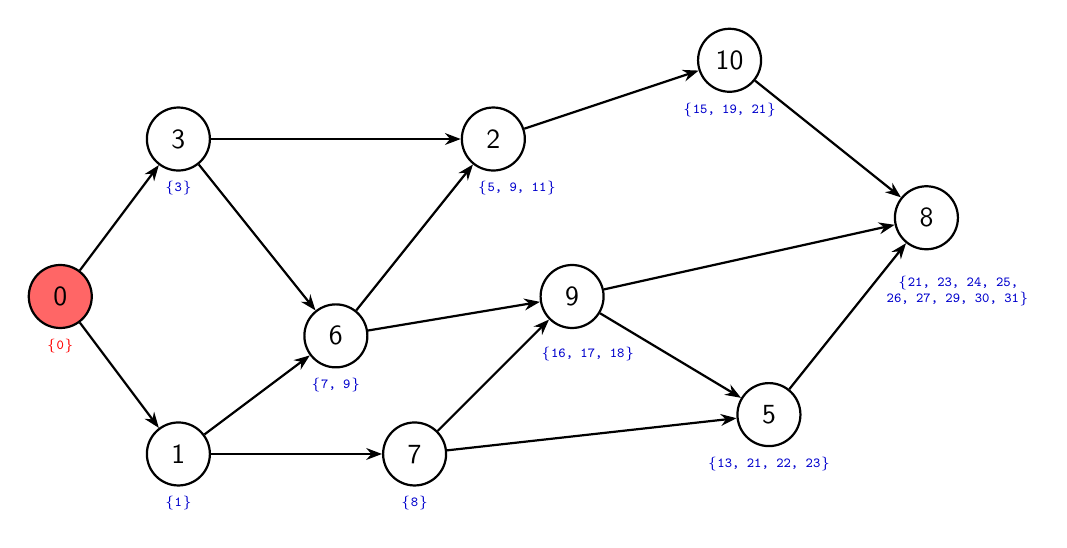
\begin{tikzpicture}[
                node distance=1.5cm and 1cm,
                base_node/.style={circle, draw=black, thick, minimum size=8mm, inner sep=0pt, font=\sffamily},
                root_node/.style={base_node, fill=red!60, text=black},
                % Definizione stile per label O-set
                data_label/.style={font=\tiny\ttfamily, text=blue!80!black, anchor=north},
                edge_style/.style={->, >={Stealth[length=2mm]}, thick, draw=black}
                ]

                % Nodes (pesi dentro)
                \node[root_node] (0) at (0, 2) {0};
                \node[base_node] (1) at (1.5, 0) {1};
                \node[base_node] (3) at (1.5, 4) {3};
                \node[base_node] (6) at (3.5, 1.5) {6};
                \node[base_node] (7) at (4.5, 0) {7};
                \node[base_node] (2) at (5.5, 4) {2};
                \node[base_node] (9) at (6.5, 2) {9};
                \node[base_node] (5) at (9, 0.5) {5};
                \node[base_node] (10) at (8.5, 5) {10};
                \node[base_node] (8) at (11, 3) {8};

                % Edges
                \draw [edge_style] (0) -- (1); \draw [edge_style] (0) -- (3);
                \draw [edge_style] (1) -- (6); \draw [edge_style] (1) -- (7);
                \draw [edge_style] (3) -- (2); \draw [edge_style] (3) -- (6);
                \draw [edge_style] (6) -- (2); \draw [edge_style] (6) -- (9);
                \draw [edge_style] (7) -- (5); \draw [edge_style] (7) -- (9);
                \draw [edge_style] (2) -- (10);
                \draw [edge_style] (9) -- (5); \draw [edge_style] (9) -- (8);
                \draw [edge_style] (10) -- (8); \draw [edge_style] (5) -- (8);

                % O-Set Labels appearing step-by-step
                \node<1->[data_label, red] at (0.south) {\{0\}};
                \node<2->[data_label] at (1.south) {\{1\}};
                \node<2->[data_label] at (3.south) {\{3\}};
                \node<3->[data_label] at (7.south) {\{8\}};
                \node<4->[data_label] at (6.south) {\{7, 9\}};
                \node<5->[data_label] at ([xshift=0.3cm]2.south) {\{5, 9, 11\}};
                \node<6->[data_label] at ([yshift=-0.1cm, xshift=0.2cm]9.south) {\{16, 17, 18\}};
                \node<7->[data_label] at (10.south) {\{15, 19, 21\}};
                \node<8->[data_label] at (5.south) {\{13, 21, 22, 23\}};
                \node<9->[data_label, align=center] at ([yshift=-0.2cm, xshift=0.4cm]8.south) {\{21, 23, 24, 25, \\ 26, 27, 29, 30, 31\}};

            \end{tikzpicture}
        } % End resizebox
    \end{figure}
\end{frame}

% --- SLIDE 15: The Rank Query - Concept ---
\begin{frame}{The Rank Query on Weighted DAGs}
    \framesubtitle{What Values are "Active" at Node N?}
    % \begin{block}{Motivation}
    %     The $\mathcal{O}$-Set ($\mathcal{O}_N$) tells us the \alert{final} path weights ending at node $N$.
    %     But we want to know which cumulative weight values are relevant \alert{during} the "processing" step associated with node $N$ itself.
    % \end{block}
    \begin{block}{Rank Query on a Node $N$: $\mathrm{rank}_G(N)$}
        \begin{enumerate}
            \item Returns a representation of a set of integers derived from the $\mathcal{O}$-set $\mathcal{O}_N$.
                  \[ S_N = \bigcup_{x \in \mathcal{O}_N} \{ z \in \mathbb{N}_0 \mid \max(0, x - w(N) + 1) \le z \le x \}. \]
                  \vspace{-1em}
                  \pause
            \item These intervals are then maximally merged. The query $\mathrm{rank}_G(N)$ returns a \alert{minimal collection of disjoint closed integer intervals}
                  \[ \mathcal{R}_N = \{[l_1, r_1], [l_2, r_2], \dots, [l_p, r_p]\} \]
                  such that their union exactly covers $S_N$.
                  % \item Return the result as a \alert{minimal set of disjoint intervals} $\mathcal{R}_N$.
        \end{enumerate}
    \end{block}
    $\mathcal{R}_N$ captures the range of possible cumulative sums during the \emph{activity} at node $N$

\end{frame}


% \subsection{Succinct Structure and Queries}
% --- SLIDE 16: The Challenge and The Core Idea ---
% \begin{frame}{The Challenge: Storing Path Information}
%     \framesubtitle{$\mathcal{O}$-Sets Can Be Huge!}

%     \begin{itemize}
%         \item \textbf{Problem}: The size $|\mathcal{O}_v|$ can grow very large!
%         \item \textbf{Question:} Can we represent the necessary information more compactly?
%     \end{itemize}

%     \begin{alertblock}<2->{Core Idea: Partitioning + Indirection}
%         \begin{enumerate}
%             \item<2-> Partition vertices $V$ into:
%                 \begin{itemize}
%                     \item \textbf{Explicit Vertices ($V_E$):} Typically sinks. Store their $\mathcal{O}_v$ directly.
%                     \item \textbf{Implicit Vertices ($V_I$):} All others. Do \emph{not} store $\mathcal{O}_v$ directly.
%                 \end{itemize}
%             \item<3-> For implicit $v \in V_I$, reconstruct $\mathcal{O}_v$ on-the-fly using:
%                 \begin{itemize}
%                     \item A chosen \textbf{designated successor} $\sigma(v) \in Succ(v)$.
%                     \item An \textbf{offset sequence} $\mathcal{J}_v$ stored at $v$.
%                 \end{itemize}
%         \end{enumerate}
%     \end{alertblock}

% \end{frame}


\begin{frame}{The Challenge: Storing Path Information}
    \framesubtitle{$\mathcal{O}$-Sets Can Be Huge!}

    % Problema e Domanda rimangono uguali
    \begin{itemize}
        \item \textbf{Problem}: The size $|\mathcal{O}_v|$ can grow very large!
        \item \textbf{Question:} Can we represent the necessary information more compactly?
    \end{itemize}


    \begin{alertblock}<2->{Core Idea: Partitioning + Indirection}
        Partition vertices $V$ into two types:
    \end{alertblock}
    \vspace{-1em}
    \begin{columns}[T] % T allinea al top
        \begin{column}{0.48\textwidth}
            \begin{block}<2->{1. Explicit Vertices ($V_E$)}
                \centering
                Store $\mathcal{O}_v$ directly. \\
                (\textit{Simple, but potentially large})
            \end{block}
            % \uncover<3->{\textbf{}
        \end{column}

        \begin{column}{0.48\textwidth}
            \begin{block}<2->{2. Implicit Vertices ($V_I$)}
                \centering
                Do \emph{not} store $\mathcal{O}_v$ explicitly \\
                (\textit{Reconstruct on-the-fly.})
            \end{block}
            \vspace{0.5em}
        \end{column}
    \end{columns}
    \uncover<3->{\textbf{Reconstruction for $v \in V_I$ using}:
        \begin{itemize}
            \item Designated Successor $\sigma(v)$
            \item Offset Sequence $\mathcal{J}_v$ (at $v$)
        \end{itemize}
    }
\end{frame}



% --- SLIDE 17: Successor Choice and Offset Sequence ---
\begin{frame}{Implicit Reconstruction: Successor \& Offset}
    \framesubtitle{How $V_I$ Nodes Refer to Others}

    \begin{block}{1. Designated Successor $\sigma(v)$ (for $v \in V_I$)}
        Which successor should $v$ point to?
        \textbf{Heuristic}: Choose $u = \sigma(v)$ that minimizes $|\mathcal{O}_u|$.
        \[ \sigma(v) \in \underset{u \in Succ(v)}{\operatorname{argmin}} \{ |\mathcal{O}_u| \}. \]
    \end{block}
    \begin{block}{2. Offset Sequence $\mathcal{J}_v$ (for $v \in V_I$)}
        How to get $\mathcal{O}_v$ from $\mathcal{O}_{\sigma(v)}$? Let $u=\sigma(v)$.
        \begin{itemize}
            % \item Property: We know $|\mathcal{O}_v| \le |\mathcal{O}_u|$.
            \item \textbf{Relationship}: Each element $x_k \in \mathcal{O}_v$ comes from some $y_{j_k} \in \mathcal{O}_u$ via $x_k = y_{j_k} - w(u)$.
            \item \textbf{Offset Sequence $\mathcal{J}_v$}: Stores the index $j_k$ corresponding to each $x_k$.
                  \[ \mathcal{J}_v = (j_0, j_1, \dots, j_{m-1}), \quad \text{where } m = |\mathcal{O}_v| \]
        \end{itemize}
    \end{block}

\end{frame}

% % --- SLIDE 16: Structure Example Visualized (Corrected Labels & No Resize) ---
% \begin{frame}{Structure Example Visualized}
%     \framesubtitle{Applying the Partitioning and Pointers}
%     \begin{figure}[hbtp]
%         \centering
%         \only<1>{\includegraphics[width=0.9\textwidth]{../bachelor-thesis/TeX/assets/succinct-dag1.pdf}}
%         \only<2>{\includegraphics[width=0.9\textwidth]{../bachelor-thesis/TeX/assets/succinct-dag2.pdf}}
%     \end{figure}
% \end{frame}

% --- SLIDE 17: Example: Computing O_7[0] (Static Structure First) ---
\begin{frame}{Example: Computing $\mathcal{O}_7[0]$}
    \framesubtitle{Following the Successor Path: $7 \to 9 \to 5 \to 8$}
    \begin{figure}[hbtp]
        \centering
        % Replace TikZ with sequential images
        \only<1>{\includegraphics[width=0.9\textwidth]{assets/dag_query1.pdf}}
        \only<2>{\includegraphics[width=0.9\textwidth]{assets/dag_query2.pdf}}
        \only<3>{\includegraphics[width=0.9\textwidth]{assets/dag_query3.pdf}}
        \only<4>{\includegraphics[width=0.9\textwidth]{assets/dag_query4.pdf}}
    \end{figure}
\end{frame}

% --- SLIDE 18: Example: Computing O_7[0] (Dynamic Structure) ---
\begin{frame}{Succinct Data Structure: Components}
    \framesubtitle{Arrays Indexed by Vertex ID}
    % divide in two columns
    \begin{columns}[T]
        \column{0.5\textwidth}
        \uncover<1->{\begin{center}
                \textbf{Each node stores 3 components}
            \end{center}
            \begin{center}
                \includegraphics[width=0.55\textwidth]{assets/AoS.pdf}
            \end{center}}

        \column{0.5\textwidth}
        \uncover<2->{\begin{center}
                \textbf{Succinct DAG as a Struct of Arrays}
            \end{center}
            \begin{center}
                \vspace{0.5em}
                \includegraphics[width=0.8\textwidth]{assets/SoA.pdf}
            \end{center}}
    \end{columns}
\end{frame}


% \subsection{Querying}
% % --- SLIDE 26: Reconstructing O-Set Elements: The Idea ---
% \begin{frame}{Reconstructing $\mathcal{O}$-Set Elements}
%     \framesubtitle{Finding $\mathcal{O}_v[k]$ for Implicit Nodes}

%     \begin{alertblock}{How?}
%         Follow the designated successor path $\sigma(v) \to \sigma(\sigma(v)) \to \dots \to e$ until an explicit node $e$ is reached.
%     \end{alertblock}


%     \begin{itemize}
%         \item Use the stored offset sequences $\mathcal{I}$ to find the corresponding index at each step.
%         \item Accumulate the weights $w(\cdot)$ along the path.
%         \item Retrieve the value from the explicit node's $\mathcal{O}_e$ and subtract the accumulated weight.
%     \end{itemize}

%     \vspace{3ex}
%     \pause
%     Let's see an example for $\mathcal{O}_7[0]$

% \end{frame}


% % --- SLIDE 28: Computing the Rank Query (RankG) (Columns Layout) ---
% \begin{frame}{Computing the Rank Query for a Node $N$}
%     \framesubtitle{High-Level Steps}

%     \begin{columns}[c] % T aligns tops
%         % Colonna sinistra: Diagramma di flusso
%         \begin{column}{0.65\textwidth}
%             \centering % Center the diagram within the column
%             \begin{tikzpicture}[node distance=1cm, auto, >=latex,
%                     box/.style={rectangle, draw, thick, text centered, minimum height=2em, minimum width=4.5cm, font=\sffamily}, % Slightly wider boxes
%                     arrow/.style={->, thick}]

%                 % Overlay on nodes to make them appear one by one
%                 \node<1-> [box] (step1) {1. Compute $\mathcal{O}_N$};
%                 \node<2-> [box, below=of step1] (step2) {2. Generate Intervals $I_x$};
%                 \node<3-> [box, below=of step2] (step3) {3. Sort Intervals};
%                 \node<4-> [box, below=of step3] (step4) {4. Merge Intervals};
%                 % Result node appears with the last arrow
%                 \node<5-> [right=1.5cm of step4] (result) {\alert{$\textsf{rank}_G(N)$}};

%                 % Overlay on arrows to match the next step appearing
%                 \draw<2-> [arrow] (step1) -- (step2);
%                 \draw<3-> [arrow] (step2) -- (step3);
%                 \draw<4-> [arrow] (step3) -- (step4);
%                 \draw<5-> [arrow] (step4) -- (result);
%             \end{tikzpicture}
%         \end{column}

%         % Colonna destra: Reminder
%         \begin{column}{0.35\textwidth}
%             \uncover<2->{ % This block appears at step 4
%                 \begin{alertblock}{Reminder}
%                     Intervals are
%                     $$I_x = [\max(0, x - w(N) + 1), x]$$
%                 \end{alertblock}
%             }
%         \end{column}
%     \end{columns}

% \end{frame}


% \subsection{Compression}
\section{Compression Strategies}
\label{sec:compression_strategies}

The succinct representation presented in \autoref{sec:succinct_dag_representation} consists of arrays for weights ($\mathcal{W}$), successor information ($\Sigma$), and associated data ($\mathcal{D}$). To further reduce the memory footprint beyond the gains achieved by the explicit/implicit node partitioning, this section discusses compression techniques for each component.

We primarily consider variable-length integer coding (\autoref{sec:integer_coding}), Elias-Fano encoding (\autoref{sec:elias_fano_code}), and Run-Length Encoding (RLE), aiming to preserve efficient access needed for query evaluation (Algorithms~\ref{alg:get_value} and \ref{alg:rank_dag}), potentially using structures like the compressed integer vectors from \autoref{app:compressed_intvec_engineering}.

\subsection{Compressing Weights and Successor Information}
\label{subsec:compressing_W_Sigma}

The components $\mathcal{W}$ and $\Sigma$ are arrays of integers, both without any guarantee of monotonicity or specific distribution patterns a priori.
\begin{itemize}
    \item $\mathcal{W}$: An array of length $n = |V|$, where $\mathcal{W}[v] = w(v) \in \mathbb{N}_0$. The values are non-negative integers representing vertex weights.
    \item $\Sigma$: An array of length $n$, where $\Sigma[v]$ stores either the integer ID $\sigma(v) \in \{0, \dots, n-1\}$ if $v \in V_I$, or a special marker (which can also be represented as an integer) if $v \in V_E$.
\end{itemize}

% Given that both $\mathcal{W}$ and $\Sigma$ are sequences of integers, the variable-length integer coding schemes discussed in \autoref{sec:integer_coding} are natural candidates for compression. Techniques such as Unary, Elias Gamma/Delta, or Rice codes can be employed. The optimal choice depends heavily on the empirical distribution of the weights $w(v)$ and the successor IDs $\sigma(v)$ (and the chosen marker value) within the specific DAG instance.

% A practical approach to implement this compression while preserving the necessary random access capability (i.e., efficiently retrieving $\mathcal{W}[v]$ or $\Sigma[v]$ for any $v$) is provided by the engineered \textsf{compressed-intvec} structure described in \autoref{app:compressed_intvec_engineering}. This structure allows selecting an appropriate integer codec (e.g., Gamma, Delta, Rice) based on the data distribution and employs a sampling mechanism to ensure $O(1)$ expected time access to any element $v$, at the cost of a typically sub-linear space overhead for the samples.

% Alternatively, if the range of possible integer values in $\mathcal{W}$ or $\Sigma$ (i.e., the maximum weight or $n$) is sufficiently small to be considered a small alphabet $\alpha$, one could choose to use Wavelet Trees (\autoref{sec:wavelet_trees}), particularly efficient variants like Wavelet Matrices or Quad Wavelet Trees (\autoref{sec:wavelet_matrices_and_quad_vectors}). These structures provide efficient Access (retrieving the element at a given position) in $O(\log \alpha)$ time, where $\alpha$ is the size of the alphabet (the number of distinct values). However, for general graphs where weights or vertex counts $n$ can be large, the alphabet size may not be small, making direct integer coding via \textsf{compressed-intvec} a more generally applicable starting point.

Since both $\mathcal{W}$ and $\Sigma$ are integer sequences, variable-length coding schemes from \autoref{sec:integer_coding} (e.g., Unary, Elias Gamma/Delta, Rice codes) are applicable. The choice of the best code depends on the observed distribution of weights and successor IDs.

To combine compression with efficient random access (retrieving $\mathcal{W}[v]$ or $\Sigma[v]$), the \textsf{compressed-intvec} structure (\autoref{app:compressed_intvec_engineering}) is a suitable implementation choice. It allows selecting an appropriate integer codec and uses sampling to achieve constant expected time access, with sub-linear space overhead for samples.

Alternatively, if the range of values (maximum weight or $n$) is small, treating them as symbols from a small alphabet $\alpha$ allows using Wavelet Trees (\autoref{sec:wavelet_trees}) or related structures (\autoref{sec:wavelet_matrices_and_quad_vectors}). These offer $O(\log |\alpha|)$ access time. However, for general graphs with potentially large weights or vertex counts, direct integer coding via \textsf{compressed-intvec} is often more practical.

\subsection{Compressing Associated Data Sequences}
\label{subsec:compressing_associated_data_sequences}

The associated data component $\mathcal{D}$ stores sequences that encode path weight information. Specifically, for an explicit vertex $v \in V_E$, $\mathcal{D}[v]$ holds the $\mathcal{O}$-set $\mathcal{O}_v = (x_0, \dots, x_{m-1})$, and for an implicit vertex $v \in V_I$, it holds the offset sequence $\mathcal{I}_v = (j_0, \dots, j_{m-1})$. Both $\mathcal{O}_v$ and $\mathcal{I}_v$ are sequences of non-negative integers which are strictly increasing ($x_k < x_{k+1}$ and $j_k < j_{k+1}$ respectively), as established by their definitions and construction rules.

This strictly monotonic property makes these sequences suitable for specialized compression techniques. Elias-Fano encoding (\autoref{sec:elias_fano_code}), discussed previously, is a strong candidate offering both good compression ratios and efficient support for operations like random access. An alternative approach, particularly effective when sequences contain long stretches of consecutive integers, is Run-Length Encoding (RLE). We detail the RLE representation below.

\subsubsection*{Run-Length Encoding (RLE) Representation}
Run-Length Encoding compresses a monotonic sequence by identifying and representing consecutive values efficiently. Consider a generic strictly increasing sequence $Y = (y_0, y_1, \dots, y_{m-1})$. A \emph{run} is a maximal contiguous subsequence $(y_i, y_{i+1}, \dots, y_{i+l-1})$ where each element is exactly one greater than its predecessor ($y_{j+1} = y_j + 1$ for $i \le j < i+l-1$). A run can have length $l=1$. RLE represents the sequence $Y$ by encoding each run using its starting value and its length.

The RLE process generates two auxiliary sequences:
\begin{itemize}
    \item The \emph{run starts sequence}, $S = (s_1, s_2, \dots, s_p)$, contains the first value $s_i$ of the $i$-th run in $Y$. Since runs are maximal and $Y$ is strictly increasing, $S$ is also strictly increasing.
    \item The \emph{run lengths sequence}, $L = (l_1, l_2, \dots, l_p)$, contains the length $l_i \ge 1$ of the $i$-th run. $L$ is a sequence of positive integers with no other guaranteed properties.
\end{itemize}
The pair $(S, L)$ allows for the exact reconstruction of $Y$. Algorithm \ref{alg:rle_encode} outlines the procedure to compute $S$ and $L$ from $Y$.

\begin{algorithm}[htbp]
    \caption{$\textsc{EncodeRLE}(Y)$: RLE encoding of a monotonic sequence}
    \label{alg:rle_encode}
    \small
    \begin{algorithmic}[1]
        \Require Monotonic sequence $Y = (y_0, y_1, \dots, y_{m-1})$, where $m = |Y|$.
        \Ensure Run starts sequence $S$, Run lengths sequence $L$.
        \State Initialize $S \leftarrow \emptyset$, $L \leftarrow \emptyset$.
        \If{$m = 0$}
        \State \Return $(S, L)$
        \EndIf
        \State $i \leftarrow 0$
        \While{$i < m$}
        \State $current\_start \leftarrow y_i$
        \State $current\_length \leftarrow 1$
        \While{$i + 1 < m$ and $y_{i+1} = y_i + 1$}
        \State $current\_length \leftarrow current\_length + 1$
        \State $i \leftarrow i + 1$
        \EndWhile
        \State Append $current\_start$ to $S$.
        \State Append $current\_length$ to $L$.
        \State $i \leftarrow i + 1$
        \EndWhile
        \State \Return $(S, L)$
    \end{algorithmic}
\end{algorithm}

The space efficiency of RLE relies on effectively compressing the resulting sequences $S$ and $L$.
The run starts sequence $S = (s_1, \dots, s_p)$ is strictly monotonic. Consequently, it is an ideal candidate for Elias-Fano encoding (\autoref{sec:elias_fano_code}).

The run lengths sequence $L = (l_1, \dots, l_p)$ is a sequence of positive integers without guaranteed structure. Standard variable-length integer codes (\autoref{sec:integer_coding}), such as Elias Gamma or Delta codes, can be applied. In practice, employing a structure like the \textsf{compressed-intvec} (\autoref{app:compressed_intvec_engineering}) allows choosing an appropriate codec and provides efficient random access.

\subsubsection*{Random Access with RLE Sequences}
Retrieving the element $y_k$ (the element at index $k$ in the original sequence $Y$, $0 \le k < m$) from the RLE representation $(S, L)$ requires identifying the run to which $y_k$ belongs. This necessitates finding the unique run index $i^*$ (where $1 \le i^* \le p$) such that:
\[ \sum_{j=1}^{i^*-1} l_j \le k < \sum_{j=1}^{i^*} l_j \]
where the sum is defined as $0$ if $i^*=1$. Once $i^*$ is found, the value $y_k$ is given by:
\[ y_k = s_{i^*} + \left( k - \sum_{j=1}^{i^*-1} l_j \right) \]
Computing the prefix sums $\sum l_j$ on the fly requires iterating through $L$, potentially leading to $O(p)$ time complexity for access, which is inefficient if the number of runs $p$ is large.

To accelerate random access, one can precompute and store the sequence of prefix sums of the run lengths:
\[ P = (p_1, p_2, \dots, p_p) \qquad  p_i = \sum_{j=1}^{i} l_j. \]
Since $l_j \ge 1$ for all $j$, the sequence $P$ is strictly increasing. As a strictly monotonic sequence, $P$ itself can be compressed effectively, for instance, using Elias-Fano encoding.

With the prefix sum sequence $P$ available, finding the index $i^*$ corresponding to the query index $k$ reduces to searching for the smallest $i^*$ such that $p_{i^*} > k$. This is a successor search problem on the monotonic sequence $P$. Using binary search on $P$ (if stored as an array) takes $O(\log p)$ time. If $P$ is stored in a structure supporting faster searches (like rank/select structures built upon certain Elias-Fano constructions), this lookup time might be further improved. Algorithm \ref{alg:rle_get_value} formalizes access using prefix sums.

\begin{algorithm}[htbp]
    \caption{$\textsc{GetValueRLE}(S, L, P, k)$: Retrieve element from RLE} % Renamed for clarity
    \label{alg:rle_get_value}
    \small
    \begin{algorithmic}[1]
        \Require $S=(s_1,\dots,s_p)$, $L=(l_1,\dots,l_p)$, $P=(p_1, \dots, p_p)$, $k \in [0, m-1]$.
        \Ensure The value $y_k$ of the element at index $k$.
        \State Find smallest $i^* \in \{1, \dots, p\}$ such that $P[i^*] > k$.
        \If{$i^* = 1$}
        \State $previous\_cumulative\_length \leftarrow 0$
        \Else
        \State $previous\_cumulative\_length \leftarrow P[i^*-1]$
        \EndIf
        \State $offset \leftarrow k - previous\_cumulative\_length$
        \State $start\_value \leftarrow S[i^*]$
        \State \Return $start\_value + offset$
    \end{algorithmic}
\end{algorithm}

\subsubsection*{Choosing Between Elias-Fano and RLE}
The choice between direct Elias-Fano encoding and Run-Length Encoding (RLE) for representing the strictly increasing sequences $\mathcal{O}_v$ and $\mathcal{I}_v$ depends on their structure. RLE is advantageous when the sequence exhibits significant clustering, meaning the number of runs $p$ is substantially smaller than the total number of elements $m$ ($p \ll m$). In such cases, the combined compressed size of the run starts $S$ and run lengths $L$ (and potentially the prefix sums $P$) might be less than direct Elias-Fano encoding of the original sequence.

On the other hand, if sequences are sparse or lack significant runs ($p$ is close to $m$), direct Elias-Fano is likely more straightforward and potentially more space-efficient.

Regardless of the chosen compression method, representing the entire associated data component $\mathcal{D}$ practically involves concatenating the compressed representations of all sequences ($\{\mathcal{D}_E(v)\}_{v \in V_E}$ and $\{\mathcal{D}_I(v)\}_{v \in V_I}$) into a single buffer. An auxiliary index structure is then needed to map each vertex ID $v$ to the starting position and metadata of its compressed sequence. The space overhead for this index is typically negligible compared to the compressed data itself


% \subsection{Achieving Sub-Entropy Space for Path Queries}
% --- SLIDE 20: Baseline: Graph Entropy H0(G) ---
\begin{frame}{Space Efficiency: Baseline Comparison}
    \framesubtitle{How Much Information is in the Graph?}
    To evaluate our structure's space, \alert{we need a baseline}.
    \begin{block}<1->{$0^{th}$-Order Graph Entropy $H_0(G)$}
        A theoretical lower bound for storing the \emph{entire} weighted DAG ($V, E, w$) losslessly.
        \[ H_0(G) = \underbrace{H_W(G)}_{\text{Cost for Weights}} + \underbrace{H_E(G)}_{\text{Cost for Topology (Edges)}} \]
    \end{block}
    \begin{itemize}
        \item<2-> $H_W(G) \approx \sum_{v \in V} \log(w(v)+1)$ bits (\emph{Minimal binary encoding for weights}).
        \item<3-> $H_E(G) \approx \log \binom{n(n-1)}{m}$ bits (\emph{Cost to choose $m=|E|$ edges out of all possible $n(n-1)$}).
    \end{itemize}
    \vspace{0.5em}
    \uncover<4->{\textbf{Any method saving the \emph{full} graph structure needs at least $H_0(G)$ bits!}}

\end{frame}


% --- SLIDE 21: Space Comparison - Key Numbers ---
\begin{frame}{Space Comparison: Succinct Structure vs. Baselines}
    \framesubtitle{Bitcoin DAG Example ($n \approx 22k, m \approx 50k$)}
    \begin{columns}[c] % Keep [t] for top alignment
        \begin{column}{0.5\textwidth} % Adjusted width potentially
            \centering
            \begin{tabular}{l r}
                \toprule
                \textbf{Method}                       & \textbf{Estimated Bits}          \\
                \midrule
                \textbf{Theoretical Lower Bound}      & \uncover<1->{\textbf{1,525,730}} \\
                \quad Weights $H_W(G)$                & \uncover<1->{60,824}             \\
                \quad Topology $H_E(G)$               & \uncover<1->{1,464,906}          \\
                \midrule
                \textit{Precomputed Rank Queries:}    &                                  \\
                \quad Explicit Binary Storage         & \uncover<2->{4,854,533}          \\
                \quad Elias-Fano Compressed           & \uncover<2->{2,211,849}          \\
                \midrule
                \textbf{Our Succinct DAG}             & \uncover<3->{\textbf{602,808}}   \\
                \quad Weights $\mathcal{W}$           & \uncover<3->{60,824}             \\
                \quad Successors $\Sigma$             & \uncover<3->{297,700}            \\
                \quad Assoc. Data $\mathcal{D}$ (RLE) & \uncover<3->{244,284}            \\
                \bottomrule
            \end{tabular}
            % Removed \end{center}
        \end{column}
        \begin{column}{0.5\textwidth} % Adjusted width to sum to 1.0
            % \begin{alertblock}<4->{Key Result}
            %     Our structure ($S(G)$) is $\approx$ \textbf{2.5x smaller} than the theoretical lower bound ($H_0(G)$) and $\approx$ \textbf{3.7x smaller} than compressed precomputation.
            % \end{alertblock}
            \begin{alertblock}<4->{Achieving Sub-Entropy Space: How?}
                Our structure is \textbf{lossy} regarding the full graph topology:
                \begin{itemize}
                    \item It \alert{does not store} the complete edge set.
                    \item It only stores the chosen successor $\sigma(v)$ for each implicit node (in $\Sigma$).
                \end{itemize}
                However, it is \textbf{lossless} for computing the specific \alert{Rank Query}.
            \end{alertblock}
        \end{column}
    \end{columns}
\end{frame}


% % --- SLIDE 22: Achieving Sub-Entropy Space: Why? (Corrected TikZ) ---
% \begin{frame}{Achieving Sub-Entropy Space: How is it Possible?}
%     \framesubtitle{Targeted Information Retention}

%     Why can our structure $S(G)$ use less space than the graph entropy $H_0(G)$?


%     \begin{center}
%         \begin{tikzpicture}[node distance=1cm, auto, >=latex,
%                 box/.style={rectangle, draw, thick, text centered, minimum height=3em, font=\sffamily, minimum width=5.5cm, align=center}, % Adjusted size and added align
%                 arrow/.style={->, thick}]

%             % Left Box: H0(G) stores the full Edge set E
%             \node [box, fill=red!10] (H0) {$H_0(G)$: Encodes \\ Full Graph $(V, \mathbf{E}, w)$};

%             % Right Box: S(G) stores only Successor info Sigma
%             \node [box, fill=green!10, right=2cm of H0] (SG) {$S(G)$: Encodes \\ $(\mathcal{W}, \Sigma, \mathcal{D})$};

%             % Labels above boxes
%             \node [above=0.3cm of H0, text width=5.5cm, align=center] {\small \textbf{Lossless Graph Encoding}};
%             \node [above=0.3cm of SG, text width=5.5cm, align=center] {\small \textbf{Our Succinct Structure}};

%         \end{tikzpicture}
%     \end{center}

%     \begin{alertblock}<1->{The Reason: Lossy Topology}
%         Our structure is \textbf{lossy} regarding the full graph topology:
%         \begin{itemize}
%             \item It \alert{does not store} the complete edge set $E$.
%             \item It only stores the chosen successor $\sigma(v)$ for each implicit node (in $\Sigma$).
%         \end{itemize}
%         However, it is \textbf{lossless} for computing the specific \alert{Rank Query}.
%     \end{alertblock}
%     % \uncover<2->{It retains only the information necessary for the target query, discarding unused topological details.}
% \end{frame}


% \section{Conclusion and Next Steps}
% --- SLIDE 23: Future Direction: Bounded Query Time ---
\begin{frame}{Future Direction: Bounded Query Time}
    \framesubtitle{Guaranteeing Predictable Performance}
    \begin{block}<1->{Performance Consideration}
        Query time for implicit node $v$ depends on the length of the successor path
        \vspace{-0.3em}
        \[v \to \sigma(v) \to \sigma(\sigma(v)) \to \dots \to e \in V_E\]
        \textbf{Problem:} Can be large/variable in deep DAGs $\implies$ slow worst-case query time.
    \end{block}
    \begin{alertblock}<2->{Solution, Challenges \& Trade-offs}
        \begin{itemize}
            \item \textbf{Solution:} Ensure every implicit node can reach an explicit node within \alert{$k$ steps}.
            \item \textbf{Challenges:} Finding the smallest possible $V'_E$ that satisfies this condition is NP-hard (\emph{minimum distance-k dominating set}).
            \item \textbf{Trade-off:} More explicit nodes $\implies$ faster queries, but larger space.
        \end{itemize}
    \end{alertblock}
\end{frame}

\backmatter

% QUESTIONS?
\begin{frame}[noframenumbering]{Worst-Case $\mathcal{O}$-Set Size: Is Exponential Growth Possible?}
    \framesubtitle{Understanding the $\mathcal{O}$-set Size}

    \begin{block}{Exponential Growth Can Occur}
        The cardinality of an $\mathcal{O}$-set, $|\mathcal{O}_v|$, is not generally bounded by a polynomial in the number of vertices $|V|$. It can grow exponentially.
    \end{block}

    \begin{block}{Underlying Reason: Path Count}
        The number of distinct paths from a source $s$ to a vertex $v$, denoted $|Path(s, v)|$, can itself be exponential in certain DAG structures. Since $|\mathcal{O}_v| \le |Path(s, v)|$, the potential for exponential size exists.
    \end{block}

    \pause % Optional pause

    \begin{alertblock}{Key Condition for Exponential Growth}
        The exponential potential is realized if the vertex weights $w(v)$ are assigned such that distinct paths $P_1 \neq P_2$ almost always lead to distinct cumulative weights $W(P_1) \neq W(P_2)$.
    \end{alertblock}

\end{frame}

\begin{frame}[noframenumbering]{Achieving Exponential $\mathcal{O}$-Set Size}
    \framesubtitle{A Strategy for Path Weight Uniqueness}

    Start with a DAG structure that naturally admits an exponential number of paths between two nodes. An example is a layered graph with multiple choices at each layer transition.

    \begin{alertblock}{Strategic Weight Assignment}
        Assign vertex weights $w(v)$ carefully to ensure path weight uniqueness.
        \[ w(v) = 2^k \quad \text{(using a unique exponent } k \text{ for each node)} \]
    \end{alertblock}

    \pause

    \begin{block}{Mechanism: Unique Binary Representation}
        With power-of-2 weights, the cumulative path weight $W(P) = \sum_{v \in P \setminus \{s\}} w(v)$ becomes a sum of distinct powers of 2.
        Due to the uniqueness of binary representation, different sets of nodes (i.e., different paths) produce different sums.
        Therefore, $|Path(s, v)|$ distinct paths yield $|\mathcal{O}_v| = |Path(s, v)|$ distinct weights.
    \end{block}

\end{frame}

\end{document}
